\documentclass[10pt]{article}
\usepackage[margin=0.6in]{geometry}
\usepackage{fancyhdr}
\usepackage{amsmath}
\usepackage{amssymb}
\usepackage{mathtools}
\usepackage{tikz}
\usetikzlibrary{patterns}
\usetikzlibrary{calc}
\usetikzlibrary{shapes.geometric}
\usepackage{multicol}
\usepackage{enumitem}
\usepackage{mathrsfs}
\usepackage{graphicx}
\usepackage{hyperref}
\usepackage{multicol}
\usepackage{lipsum}
\pagestyle{fancy}

\title{Metric Spaces Notes}
\author{Henry Wise}
\date{October 2023}

\begin{document}

\maketitle

\tableofcontents
\begin{multicols}{3}
\begin{itemize}
    \item Lecture 1: pages 2 - 5
    \item Lecture 2: pages 6 - 8
    \item Lecture 3: pages 9 - 11
    \item Lecture 4: pages 12 - 14
    \item Lecture 5: Pages 14 - 15
    \item Lecture 6: Pages 15 - 18
\end{itemize}
\end{multicols}
\vspace*{\fill}
\section{suggested reading}
\begin{itemize}
    \item \textbf{Metric Spaces (Springer Undergraduate Mathematics Series)}, Mícheál Ó Searcóid \cite{Book 1}
    \item \textbf{Metric Sapces}, Satish \& Harkrishan \cite{Book 2}
    \item \textbf{Guide to Analysis}, F. Mary Hart \cite{Book 3}
    \item \textbf{How to think about Analysis}, Lara Alcock \cite{Book 4}
    \item \textbf{Numbers Sequences \& Series}, Kieth E. Hirst \cite{Book 5}
\end{itemize}

\newpage

\section{Introduction to Metric Spaces}
\subsection{Whats a Metric?}
Start by using the model $\mathbb{R}^{2}$ wherein $(0,1)\subseteq\mathbb{R}$, we have that
\begin{align*}
    \mathbb{R}^{2}=\{(x,y)|x,y\in\mathbb{R}\}
\end{align*}
Let's create a function called a ``Metric" with a symbol $d$. Where
\begin{align*}
    d(\underline{x},\underline{y})=|\underline{x}-\underline{y}|,\,\,\,\,\underline{x},\underline{y}\in\mathbb{R}^{2}
\end{align*}
See that

\begin{center}
\begin{tikzpicture}[scale=4]
    \draw[->](0,0)--(2,0);
    \draw[->](0,0)--(0,1);
    \draw[-](0.25,0.25)--(1.5,0.75);
    \draw[fill, blue] (0.25,0.25) circle [radius=0.025];
    \draw[fill, red] (1.5,0.75) circle [radius=0.025];
    \node[above, scale=1.5] at (0.25,0.26) {$\underline{x}$};
    \node[above, scale=1.5] at (1.5,0.76) {$\underline{y}$};
    \node[above, scale=1.5] at (1,0.25) {$\sim d(\underline{x},\underline{y})$};
\end{tikzpicture}
\end{center}
where the essential properties of $d$ on $\mathbb{R}^{2}$ are as follows:
\begin{enumerate}
    \item $d(\underline{x},\underline{y})\geq0$,
    \item $d(\underline{x},\underline{y})=0\implies\underline{x}=\underline{y}$,
    \item $d(\underline{x},\underline{y})=d(\underline{y},\underline{x})$,
    \item The distance is the shortest distance between the 2 points. So $d(\underline{x},\underline{y})\leq d(\underline{x},\underline{z})+d(\underline{z},\underline{y})$.
\end{enumerate}

A metric $d$ is a distance function between two points in a space. There are lots of different types of metrics for all different kinds of spaces. The standard Metric or ``Euclidean Metric" for $\mathbb{R}$ is
\begin{align*}
    d(x,y)=|x-y|.
\end{align*}

\subsection{Whats a Metric Space?}
The abstract definition of a metric space. Let $X$ be a non-empty set. A metric on $X$ is a function $d:X\times X\to[0,\infty)$ satisfying:
\begin{align*}
    \textbf{M1)}&\,\,d(x,y)\geq0\\
    \textbf{M2)}&\,\,d(x,y)=0\implies x=y\\
    \textbf{M3)}&\,\,d(x,y)=d(y,x)\\
    \textbf{M4)}&\,\,d(x,y)\leq d(x,z)+d(z,y)\text{ (triangle inequality)}\\
    &\forall x,y,z\in X.
\end{align*}

The pair $(X,d)$ is the metric space of $X$ with a metric $d$. Note that $X$ is just a set, it needs an associated metric ``$d$" in order to become a metric space.

\subsubsection{Examples of Metric Spaces}
\begin{enumerate}
    \item The trivial metric on a set. Take $X\neq\emptyset$, define the function $\delta:X\times X\to[0,\infty)$ by
    \begin{equation*}
        \delta(x,y)=
        \begin{cases}
            0 & \text{if $x=y$}\\
            1 & \text{if $x\neq y$}
        \end{cases}
    \end{equation*}
    To show it is a metric on $X$ we need only verify the axioms of a metric.
    \begin{enumerate}
        \item Take arbitrary $x,y,z\in X$, then $\delta(x,y)\in~\{0,1\}$ so \textbf{M1} holds. 
        \item Suppose $x=y$, then by definition $\delta(x,y)=0$. Furthermore if $x\neq y$ then $\delta(x,y)=1\neq0$ so \textbf{M2} holds. 
        \item Now take $x,y\in X$. If $x=y$ then $\delta(x,y)=0=\delta(y,x)$ and if $x\neq y$ then $\delta(x,y)=1=\delta(y,x)$ so $\delta(x,y)=\delta(y,x)$ so \textbf{M3} holds.
    \end{enumerate}
    All that's left now is to verify the triangle inequality (often the hardest part).

    (d) Take $x,y,z\in X$. Then $\delta(x,y)\leq1$, $\delta(x,z)\leq1$ and $\delta(z,y)\leq1$. If $x=y$ then $\delta(x,y)=0\leq \delta(x,z)+\delta(z,y)$ as $\delta(x,z),\,\delta(z,y)\geq0$. If $x\neq y$ then $\delta(x,y)=1$. Now $z$ could equal $x$, but if it does then it cannot be equal to $y$ and $\delta(z,y)=1$. If $z=y$ then $z\neq x\implies\delta(x,z)=1$. In both, $\delta(x,y)=1\leq1=\delta(x,z)+\delta(z,y)$. All that is left is if $z\neq x,y$. So $\delta(x,z)+\delta(z,y)=2>1$. Therefore the triangle equality is conserved and \textbf{M4} holds.

    Consider $\mathbb{R}$ equipped with the metric $\delta$. What real numbers lie in the set $\{x\in\mathbb{R}\,|\,\delta(x,0)<1\}$? In this event, 0 would be the only such element.
    \begin{align*}
        \{x\in\mathbb{R}\,|\,\delta(x,0)<1\}=\{0\}.
    \end{align*}

    What about the real numbers that lie in the set $\{x\in\mathbb{R}\,|\,\delta(x,0)\leq1\}$? Every single real number satisfies this set!
    \begin{align*}
        \{x\in\mathbb{R}\,|\,\delta(x,0)\leq1\}=\mathbb{R}
    \end{align*}

    \item The standard metric on $\mathbb{R}$. The metric $d:\mathbb{R}\times\mathbb{R}\to[0,\infty)$ where
    \begin{align*}
        d(x,y)=|x-y|.
    \end{align*}
    Which follows all the axioms of a metric
    \begin{enumerate}
        \item $d(x,y)\geq0$ by definition \textbf{(M1)}
        \item If $x=y$ then $d(x,y)=|x-y|=0$. Furthermore if $d(x,y)=0$ then $|x-y|=0\implies x=y$. \textbf{(M2)}
        \item $d(x,y)=|x-y|=|y-x|=d(y,x)$ \textbf{(M3)}
        \item To show that $|x-y|=d(x,y)\leq d(x,z)+d(z,y)=|x-z|+|z-y|$. As we know that $d(x,y)\geq0$, $d(x,z)\geq0$ and $d(z,y)\geq0$. If $x=y$ then $d(x,y)=0\leq d(x,z)+d(z,y)$. If $x\neq y$ then we can have $z=x$, then $|x-y|=|x-x|+|x-y|=|x-y|$, or $z=y$ and $|x-y|=|x-y|+|y-y|$. If $z\neq x, y$ then we have $|x-z|+|z-y|\geq|x-z+z-y|=|x-y|$ by the \emph{triangle inequality}. So all cases are satisfied and the triangle inequality holds. \textbf{(M4)}
    \end{enumerate}

    \boxed{\text{Note: Unless otherwise stated, this is the metric used in a space. Hence it being ``standard".}}

    \item Case study in $\mathbb{R}^{2}$. \emph{Used for the next few examples also!}

    Three different metrics in $\mathbb{R}^{2}$:
    \begin{enumerate}
        \item $d_{1}:\mathbb{R}^{2}\times\mathbb{R}^{2}\to[0,\infty)$
        \begin{align*}
            d_{1}(x,y)=|x_{1}-y_{1}|+|x_{2}-y_{2}|
        \end{align*}
        \item $d_{2}:\mathbb{R}^{2}\times\mathbb{R}^{2}\to[0,\infty)$
        \begin{align*}
            d_{2}(x,y)=\sqrt{(x_{1}-y_{1})^{2}+(x_{2}-y_{2})^{2}}
        \end{align*}
        This is the standard metric in $\mathbb{R}^{2}$

        \item $d_{\infty}:\mathbb{R}^{2}\times\mathbb{R}^{2}\to[0,\infty)$
        \begin{align*}
            d_{\infty}(x,y)=\max\{|x_{1}-y_{1}|,\,|x_{2}-y_{2}|\}
        \end{align*}
    \end{enumerate}
    Throughout the above, we have that $x=(x_{1}, x_{2})$ and $y=(y_{1}, y_{2})$.

    \begin{center}
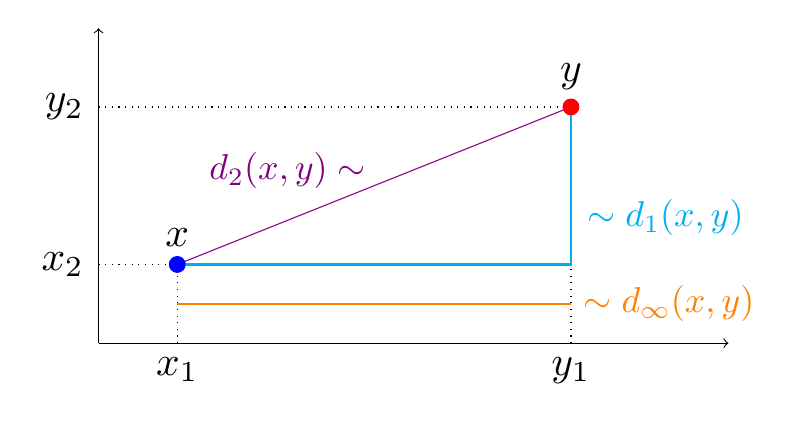
\begin{tikzpicture}[scale=4]
    \draw[->](0,0)--(2,0);
    \draw[->](0,0)--(0,1);
    \draw[-, violet](0.25,0.25)--(1.5,0.75);
    \node[above, scale=1.5] at (0.25,0.26) {$x$};
    \node[above, scale=1.5] at (1.5,0.76) {$y$};
    \node[above, scale=1.3, violet] at (0.6,0.45) {$d_{2}(x,y)\sim$};
    \draw[dotted](0.25,0)--(0.25,0.25);
    \draw[dotted](0,0.25)--(0.25,0.25);
    \draw[dotted](0,0.75)--(1.5,0.75);
    \draw[dotted](1.5,0)--(1.5,0.75);
    \node[below, scale=1.5] at (0.25,0) {$x_{1}$};
    \node[left, scale=1.5] at (0,0.25) {$x_{2}$};
    \node[below, scale=1.5] at (1.5,0) {$y_{1}$};
    \node[left, scale=1.5] at (0,0.75) {$y_{2}$};
    \draw[-, cyan, thick](0.25,0.25)--(1.5,0.25)--(1.5,0.75);
    \node[above, scale=1.3, cyan] at (1.8,0.3) {$\sim d_{1}(x,y)$};
    \draw[-, orange, thick](0.25,0.125)--(1.5,0.125);
    \node[right, scale=1.3, orange] at (1.5,0.125) {$\sim d_{\infty}(x,y)$};
    \draw[fill, blue] (0.25,0.25) circle [radius=0.025];
    \draw[fill, red] (1.5,0.75) circle [radius=0.025];
\end{tikzpicture}
\end{center}
\end{enumerate}

\subsubsection{What is a Unit Circle?}
Consider what the ``Unit Circle" would look like in $(\mathbb{R}^{2}, d_{1})$, $(\mathbb{R}^{2}, d_{2})$ and $(\mathbb{R}^{2}, d_{\infty})$. That is $S_{i}^{1}$ where $i=1,2,\infty$ or $S_{i}^{1}=\{x\in\mathbb{R}\,|\,d_{i}(x,0)=1\}$:
\begin{itemize}
    \item $S_{2}^{1}$:
    \begin{multicols}{2}
    \begin{tikzpicture}[scale=2]
        \draw[->](-1.5,0)--(1.5,0);
        \draw[->](0,-1.5)--(0,1.5);
        \draw[-] (0,0) circle [radius=1];
    \end{tikzpicture}

    \begin{align*}
        S_{2}^{1}=\{x\in\mathbb{R}\,|\,d_{2}(x,0)=1\}=\{x\in\mathbb{R}:\sqrt{x_{1}^{2}+x_{2}^{2}}=1\}
    \end{align*}
    The Unit circle in $S_{1}^{1}$ is exactly what you would expect a Unit circle to look like. Constant radius all around. This is because we're using the standard metric, which is one that we've been using for most of our academic career (Up till now of course). Note that this is called a circle, not a ball! This is important later. 
    \end{multicols}

    \item $S_{\infty}^{1}$:
    \begin{multicols}{2}
    \begin{tikzpicture}[scale=2]
        \draw[->](-1.5,0)--(1.5,0);
        \draw[->](0,-1.5)--(0,1.5);
        \draw[-](1,1)--(1,-1)--(-1,-1)--(-1,1)--(1,1);
    \end{tikzpicture}

    \begin{align*}
        S_{\infty}^{1}=\{x\in\mathbb{R}\,|\,d_{\infty}(x,0)=1\}=\{x\in\mathbb{R}:\max\{|x_{1}|,|x_{2}|\}=1\}
    \end{align*}
    Suppose $x=(x_{1},1)$, then 
    \begin{align*}
        d_{\infty}(x,0)&=\max\{|x_{1}-0|,\,|1-0|\}\\
        &=\max\{|x_{1}|,1\}\\
        &=1 \text{ if } -1\leq x_{1}\leq1
    \end{align*}
    This is also consistent for $x_{2}$ and is how we end up with the square shape.
    \end{multicols}
    
    \item $S_{1}^{1}$:
    \begin{multicols}{2}
    \begin{tikzpicture}[scale=2]
        \draw[->](-1.5,0)--(1.5,0);
        \draw[->](0,-1.5)--(0,1.5);
        \draw[-](0,1)--(1,0)--(0,-1)--(-1,0)--(0,1);
    \end{tikzpicture}

    \begin{align*}
        S_{1}^{1}=\{x\in\mathbb{R}\,|\,d_{1}(x,0)=1\}=\{x\in\mathbb{R}:|x_{1}|+|x_{2}|=1\}
    \end{align*}
    For $d_{1}(x,0)=1$ where $x=(x_{1}, x_{2})$ we need $1=x_{1}+y$ which implies that $y=1-x_{1}$ where $y$ is the absolute value.

    A good way to think about how this shape occurs would be to see what values $x_{1}$ and $x_{2}$ need to take in order for the rules of the set $S_{1}^{1}$ to be satisfied.
    For example:
    \begin{align*}
        d(x,0)&=1\\
        \implies|x_{1}|+|x_{2}|&=1 
    \end{align*}
    so if $x_{1}=1$ or $-1$, then $x_{2}=0$. And visa versa! This is where the term above arises. The equation $y=1-x_{1}$ is just another way of showing $|x_{2}|=1-|x_{1 }|$
    \end{multicols}
\end{itemize}
\newpage

\subsubsection{Real n-dimensional Metric}
While still using the three example metrics from before, consider $(\mathbb{R}^{n}, d_{1})$, $(\mathbb{R}^{n}, d_{2})$ and $(\mathbb{R}^{n}, d_{\infty})$ where $n\in\mathbb{N}\setminus\{1\}$.

So
\begin{align*}
    d_{1}(x,y)&=\sum^{n}_{i=1}|x_{i}-y_{i}|,\\
    (\star)\,d_{2}(x,y)&=\sqrt{\sum^{n}_{i=1}(x_{i}-y_{i})^{2}}
\end{align*}
($\star$) Standard or Euclidean metric on $\mathbb{R}^{n}$

\subsubsection{Proof of a real n-dimensional metric space}
For this we prove $(\mathbb{R}^{n}, d_{2})$ is a metric space.
\begin{itemize}
    \item[\textbf{M1)}] Take $x,y\in\mathbb{R}^{n}$ then $d(x,y)\geq0$ as $\sum^{n}_{i=1}(x_{i}-y_{i})^{2}\in[0,\infty)\therefore$ has a real square root.
    
    So $\sqrt{\sum^{n}_{i=1}(x_{i}-y_{i})^{2}}\geq0$ as $\sqrt{\empty}$ is assumed to be positive.

    \item[\textbf{M2)}] If $x=y$ then $x_{i}=y_{i}$ for $i=1,2,\dots,n$. So $x_{i}-y_{i}=0$ \& $(x_{i}-y_{i})^{2}=0$

    It follows then that $\sum^{n}_{i=1}(x_{i}-y_{i})^{2}=0$ \& $\sqrt{0}=0$.

    If $d_{2}(x,y=0)$ then $\sqrt{\sum^{n}_{i=1}(x_{i}-y_{i})^{2}}=0$ so $\sum^{n}_{i=1}(x_{i}-y_{i})^{2}=0$ \& $(x_{i}-y_{i})^{2}\geq0$ $\forall i\in\{1,2,\dots,n\}$

    $\therefore (x_{i}-y_{i})^{2}=0$ $\therefore x_{i}=y_{i}\,\forall i\in\{1,2,\dots,n\}$ Hence $x=y$.

    \item[\textbf{M3)}] Symmetry

    Take $x,y\in\mathbb{R}^{2}$ then $d_{2}(x,y)=\sqrt{\sum^{n}_{i=1}(x_{i}-y_{i})^{2}}=\sqrt{\sum^{n}_{i=1}(-1)^{2}(y_{i}-x_{i})^{2}}=\sqrt{\sum^{n}_{i=1}(y_{i}-x_{i})^{2}}=d_{2}(y,x)$

    \item[\textbf{M4)}] The triangle inequality

    Take $x,y\in\mathbb{R}^{2}$. Consider $d_{2}(x,z)+d_{2}(z,y)=\sqrt{\sum^{n}_{i=1}(x_{i}-z_{i})^{2}}+\sqrt{\sum^{n}_{i=1}(z_{i}-y_{i})^{2}}$
    
    let $r_{i}=|x_{i}-z_{i}|$ and $s_{i}=|y_{i}-z_{i}|$

    So $d_{2}(x,z)+d_{2}(z,y)=\sqrt{\sum^{n}_{i=1}r_{i}^{2}}+\sqrt{\sum^{n}_{i=1}s_{i}^{2}}$

    We now apply a result due to \emph{Hermann. Minkowski}, which allows us to deduce:

    $d_{2}(x,z)+d_{2}(z,y)=\sqrt{\sum^{n}_{i=1}r_{i}^{2}}+\sqrt{\sum^{n}_{i=1}s_{i}^{2}}\geq\sqrt{\sum^{n}_{i=1}(r_{i}+s_{i})^{2}}$

    But $r_{i}+s_{i}=|x_{i}-z_{i}|+|z_{i}-y_{i}|\geq|x_{i}-z_{i}+z_{i}-y_{i}|=|x_{i}-y_{i}|$

    And so $d_{2}(x,z)+d_{2}(z,y)\geq\sqrt{\sum^{n}_{i=1}(x_{i}-y_{i})^{2}}=d_{2}(x,y)$. 

    So $d_{2}(x,y)\leq d_{2}(x,z)+d_{2}(z,y)$.
\end{itemize}

\newpage

\section{Functions and Analysis of Metric Spaces}
Remember real-analysis?
\subsection{The Real Analysis: Infima \& Suprema}
Consider $I=[0,1]$, $[0,1)$, $(0,1)$. Where $[0,1]=\{t:0\leq t\leq1\}$, $[0,1)=\{t:0\leq t<1\}$ and $(0,1)=\{t:0<t<1\}$. 

Take $S\subseteq\mathbb{R}$. Then $S$ is bounded above $\iff\exists M\in\mathbb{R}$ such that $x\leq M\, \forall x\in S$

\begin{center}
    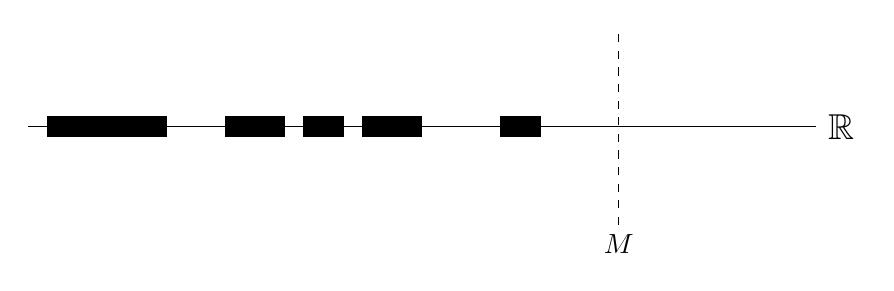
\begin{tikzpicture}[scale=2.5]
        \draw[-](0,0)--(4,0);
        \draw[dashed](3,-0.5)--(3,0.5);
        \node[right, scale=1.3] at (4,0){$\mathbb{R}$};
        \node[below] at (3,-0.5){$M$};
        \draw[fill] (0.1,-0.05) rectangle (0.7,0.05);
        \draw[fill] (1,-0.05) rectangle (1.3,0.05);
        \draw[fill] (1.4,-0.05) rectangle (1.6,0.05);
        \draw[fill] (1.7,-0.05) rectangle (2,0.05);
        \draw[fill] (2.4,-0.05) rectangle (2.6,0.05);
    \end{tikzpicture}
\end{center}

If $S$ is bounded above by $M$, then any $M'>M$ is also an upper bound. The Supremum of $S$, $\sup{S}$, is the least (or smallest) upper bound for $S$. But what does ``least" imply? If we take $\varepsilon>0$ then $\sup{(S)}-\varepsilon$ is not an upper bound.\footnote{Note: $\varepsilon+\varepsilon=\varepsilon$. ``Small plus small is small" - Jason} This means $\exists x\in S$ such that $\sup{(S)}-\varepsilon<x$. 
\begin{quote}
    Take $S=(0,1)$ then $\sup{(S)}=1$ as there is an $x\in(0,1)$ between $\sup(S)-\varepsilon$ \& 1. For example, take $1-\frac{\varepsilon}{2}$.
\end{quote}
\begin{itemize}
    \item[Fact:] There is no reason to assume $\sup(S)\in S$, if however $\sup(S)\in S$ then we say $S$ has a maximal element, denoted $\max(S)$. If $S$ has no upper bound $\exists x\in S$ for which $x>M$ for any choice of $M$ then we define $\sup(S)=\infty$.
\end{itemize}
The set $S$ is bounded below if $\exists m\in\mathbb{R}$ such that $m\leq x\,\forall x\in S$. The Infimum of $S$, $\inf{(S)}$ is the largest lower bound for $S$. Again, there is no reason for $\inf{(S)}\in S$, but if $\inf{(S)}\in S$ then $S$ has a minimum element denoted by $\min{(S)}$. If no lower bound exists then $\inf{(S)}=-\infty$.
\begin{quote}
    Take the empty set $\emptyset$; $\sup(\emptyset)=-\infty$ (The smallest upper bound) \& $\inf(\emptyset)=\infty$ (The largest lower bound). The empty set is the only case wherein the supremum is less than the infimum.
\end{quote}
But why should sup or inf even exist? The reason is that $\mathbb{R}$ has a property called completeness. $\mathbb{R}$ is complete and it satisfies the so-called completeness axiom, which states that any bounded above set in $\mathbb{R}$ which is non-empty \underline{has} a supremum. This might be the case in other settings,
\begin{quote}
    Take $x=\mathbb{Q}$ the rational numbers. We can construct a sequence of rationals $\frac{p_{n}}{q_{n}}$ such that $(\frac{p_{n}}{q_{n}})^{2}\to2$ as $n\to\infty$. Thus $\{\frac{p_{n}}{q_{n}}:n\in\mathbb{N}\}$ and 2 is an upper bound, but it has no supremum in $\mathbb{Q}$. This is because there is no rational number representation of $2^{1/2}$ or $\sqrt{2}$.
\end{quote}
If you're confident with these ideas then you will find some of the later proofs easier to understand. If not, I would recommend you try a book by Alcock L. \textbf{How to Think about Analysis}\cite{Book 4}
\subsection{Sets of sequences \& Function Spaces}
\subsubsection{Sets of sequences}
We already know that $\mathbb{R}^{n}$ is a finite-dimensional object, but what about $\mathbb{R}^{\mathbb{N}}$ (The set of all sequences of real numbers)? If $x\in\mathbb{R}^{\mathbb{N}}$ then $x=(x_{1}, x_{2}, x_{3}, \dots, x_{n}, \dots)$. We can't immediately use variants of $d_{1}$, $d_{2}$ or $d_{\infty}$. Why? As an example of exactly why, let's try to apply $d_{1}(x,0)$:
\begin{equation*}
    d_{1}(x,0)=d\Big{(}(x_{1},x_{2},\dots),(0,0,\dots)\Big{)}=\sum^{\infty}_{i=1}|x_{i}-0|=\sum^{\infty}_{i=1}|x_{i}|=\infty?
\end{equation*}
There are many sequences where the evaluation of this metric is infinite, which doesn't work for us. We need the value to be a non-negative real number.
\begin{quote}
$l_{1}$ is the set of all sequences of real numbers that satisfy $\sum^{\infty}_{n=1}|x_{i}|<\infty\,(\star)$. Take $x=(1,\frac{1}{2}, \frac{1}{4}, \dots, \frac{1}{2^{n}}, \dots)$, then $x\in l_{1}$, but if $y=(1, \frac{1}{2}, \frac{1}{3}, \dots, \frac{1}{n}, \dots)$ then $\sum^{\infty}_{n=1}|x_{n}|=\sum^{\infty}_{n=1}\frac{1}{n}=+\infty$. So $l_{1}$ is the set of all sequences satisfying $(\star)$ \& $d_{1}(x,y)=\sum^{\infty}_{n=1}|x_{n}-y_{n}|$ is the metric. 
\end{quote}
The first example of an infinite-dimensional vector space with a metric on it (A big space).
\begin{quote}
    $l_{\infty}$ is the set of all bounded sequences of real numbers; $x\in l_{\infty}\iff\exists M=M(x)>0$ such that $|x_{n}|\leq M \forall n\in\mathbb{N}$, then $d_{\infty}(x,y)=\sup\{|x_{i}-y_{i}|:i\in\mathbb{N}\}$. Note that $x-y=(x_{1}-y_{1}, x_{2}-y_{2}, \dots)\in l_{\infty}$.
\end{quote}

\subsubsection{Function Spaces}
Ideally, we would be able to apply all our theory thus far to $F(X, Y)$, the set of all functions from the set $X$ to $Y$. Look at $C([0,1])$ \& $B([0,1])$ where $C([0,1])$ is the set of all continuous functions $f:[0,1]\to\mathbb{R}$ \& $B([0,1])$ is the set of all bounded\footnote{Bounded $\implies\exists M>0$ such that $|f(x)|<M \forall x\in[0,1]$} functions $f:[0,1]\to\mathbb{R}$. Let's try to draw a couple of functions:
\begin{multicols}{2}
    \begin{tikzpicture}
        \draw[-](0,0)--(8,0);
        \draw[-](0,-1)--(0,3);
        \draw[-](0,1.8) .. controls (0.2,2.5) and (0.6,2.5) .. (0.8,1.8)--(0.8,1.8) .. controls (1,1.2) and (1.45,1) .. (
        1.5,1.8)--(
        1.5,1.8) .. controls (1.6,3) and (2.8,3) .. (2.85,1.8)--(2.85,1.8) .. controls (2.9,-1) and (3.8,-1) .. (4.1,-0.9)--(4.1,-0.9) .. controls (4.6,-0.7) and (4.4,-0.1) .. (4.6,-0.1)--(4.6,-0.1) parabola (4.7,-0.2)--(4.7,-0.2) .. controls (4.8,-0.39) and (4.9,-0.2) .. (5,1)--(5,1) .. controls (5.2,3) and (6.8,3) .. (7,1)--(7,1) .. controls (7.1,-0.5) and (7.5,-1) .. (8,-0.5);
        \draw[dotted](8,3)--(8,-1);
        \node[below] at (0,-1) {$0$};
        \node[below] at (8,-1) {$1$};
    \end{tikzpicture}

    \begin{tikzpicture}
        \draw[-](0,0)--(8,0);
        \draw[-](0,-1)--(0,3);
        \draw[-](0,0) parabola (2,2)--(2,2) .. controls (2.789,3.5) and (3.8,2.5) .. (4,2)--(4,2) .. controls (4.8,0.6) and (6.8,1) .. (8,3);
        \draw[dotted](8,3)--(8,-1);
        \node[below] at (0,-1) {$0$};
        \node[below] at (8,-1) {$1$};
    \end{tikzpicture}
\end{multicols}
\begin{multicols}{2}
    \begin{tikzpicture}
        \draw[-](0,0)--(8,0);
        \draw[-](0,-1)--(0,3);
        \draw[dotted](8,3)--(8,-1);
        \draw[-](0,0)--(4,3)--(8,0);
        \node[below] at (0,-1) {$0$};
        \node[below] at (8,-1) {$1$};
    \end{tikzpicture}

    \begin{tikzpicture}
        \draw[-](0,0)--(8,0);
        \draw[-](0,-1)--(0,3);
        \draw[-](4,1) circle [radius=0.1];
        \draw[fill](4,2) circle [radius=0.1];
        \draw[-](0,1)--(3.9,1);
        \draw[-](4,2)--(8,2);
        \draw[dotted](8,3)--(8,-1);
        \node[below] at (0,-1) {$0$};
        \node[below] at (8,-1) {$1$};
        \node[below] at (4,-0.5){$\notin C([0,1])$, but $\in B([0,1])$};
    \end{tikzpicture}
\end{multicols}
\begin{equation*}
    f[0,1]\to\mathbb{R},\,t\to
    \begin{cases}
        1 &\text{if $t\in\mathbb{Q}$}\\
        0 &\text{if $t\notin\mathbb{Q}$}
    \end{cases}
\end{equation*}
In this case, with this particular function seen in the bottom right $f\notin C([0,1])\text{ however }f\in B([0,1])$. We want to be able to put a metric on these functions. We'll start with bounded functions and we'll try the sup metric across $d_{\infty}: B([0,1])\times B([0,1])\to[0,\infty)$ where $d_{\infty}(f,g)=\sup\{|f(t)-g(t)|:t\in[0,1]\}$.
\begin{quote}
    For example: Take $f:[0,1]\to\mathbb{R}$ such that $f(t)=1$ \& take $g:[0,1]\to\mathbb{R}$ such that $g(t)=t$,
    \begin{align*}
        d_{\infty}(f,g)&=\sup\{|f(t)-g(t)|\}\\
        &=\sup\{|1-g(t)|\}\\
        &=\sup\{1-g(t)\}\\
        &=1
    \end{align*}
    The pair $\Big{(}B([0,1]),d_{\infty}\Big{)}$ is a metric space. This is a function space. And it can be verified using the axioms of a metric space. 
    \begin{enumerate}
        \item[\textbf{M1)}] $f,g$ are bounded functions with domain $[0,1]$ and co-domain $\mathbb{R}$. So $f-g$ which is the function $f-g:[0,1]\to\mathbb{R};t\to f(t)-g(t)$ and is bounded. Here, $d_{\infty}(f,g)=\sup\{\underbrace{|f(t)-g(t)|}_{\geq0}\}\leq M$ so $d_{\infty}(f,g)\geq0$ $\forall f, g$. 
        \item[\textbf{M2)}] If $f=g$ then $f(t)=g(t)$ $\forall t\in[0,1]$, so $f(t)-g(t)=0$ $\forall t\in[0,1]$ thus $|f(t)-g(t)|=0$ $\forall t\in[0,1]$ and $\sup\{0\}=0.$ If $d_{\infty}(f,g)=0\implies\sup\{|f(t)-g(t)|\}=0$ so $|f(t)-g(t)|\leq0$ $\forall t\in[0,1]$ But $|f(t)-g(t)|\geq0$ so $|f(t)-g(t)|=0$. Thus $f=g$.
        \item[\textbf{M3)}] Look at $d_{\infty}(f,g)=\sup\{|f(t)-g(t)|:t\in[0,1]\}=\sup\{|g(t)-f(t)|:t\in[0,1]\}=d_{\infty}(g,f)$
        \item[\textbf{M4)}] Take $f,g,h\in B([0,1])$, then 
        \begin{align*}
            d_{\infty}(f,g)&=\sup\{|f(t)-g(t)|:t\in[0,1]\}\\
            &=\sup\{|f(t)-h(t)+h(t)-g(t)|:t\in[0,1]\}\\
            \text{(triangle inequality) }&\leq\sup\{|f(t)-h(t)|+|h(t)-g(t)|:t\in[0,1]\}\\
            \text{(A property of sup)}&\leq\sup\{|f(t)-h(t)|:t\in[0,1]\}+\sup\{|h(t)-g(t)|:t\in[0,1]\}\\
            &=d_{\infty}(f,h)+d_{\infty}(h,g).
        \end{align*}
        
    \end{enumerate}
\end{quote}

\newpage

\section{Vector Spaces and the New Norm}
In all the examples we have considered thus far, the metric $d$ has involved a term of the form $|b-a|$ in some form. ie: Standard metric on $\mathbb{R}$:
\begin{align*}
    d_{2}(x,y)=\sqrt{\sum^{n}_{i=1}\underbrace{(x_{i}-y_{i})^{2}}_{|x_{i}-y_{i}|^{2}}}
\end{align*}
In general, a metric space need not support any algebraic structure. The definition of $d$ on $X\neq\emptyset$ makes no mention of any such structure.

\subsection{Hamming Distance}
Take a finite set $A$, say $\{\omega_{1},\omega_{2},\dots,\omega_{n}\}$, called an alphabet \& $A(N)$ is the set of all strings of length $N$. ``string": $\omega^{(1)}, \omega^{(2)}, \omega^{(3)},\dots,\omega^{(n)}$. For example: $A=\{0,1\}$, $A(3)=\{000, 001, 010, 011, 100, 101, 110, 111\}$. The Hamming distance $H:A(3)\to[0,\infty)$ is defined to be the number of places where string $x$ differs from string $y$. $H(010,110)=1$.

\subsection{Vector Spaces}
Recall $\mathbb{R}^{2}$

\begin{multicols}{2}
So a vector space is basically a non-empty set $V$ of elements that we call vectors which satisfy: $\mu\underline{u}+\lambda\underline{v}\in V$ if $\underbrace{\underline{u}, \underline{v}}_{\text{Vectors}}\in V$ \& $\underbrace{\mu, \lambda}_{\text{Scalars}}\in\underbrace{\mathbb{R}\,(\text{ or } \mathbb{C})}_{\text{Scalar Field}}$.

Abstracts $a-b$:
\begin{align*}
    \underline{u}-\underline{v}=\underline{u}+(-1)\underline{v}
\end{align*}
But we're missing the abstraction of the absolute value. The vector space version, $||\cdot||$ is called a norm.

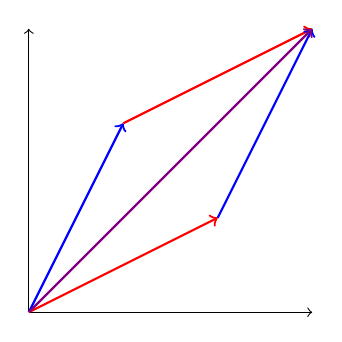
\begin{tikzpicture}[scale=1.2]
    \draw[->](0,0)--(3,0);
    \draw[->](0,0)--(0,3);
    \draw[->, blue, thick](0,0)--(1,2);
    \draw[->, red, thick](0,0)--(2,1);
    \draw[->, red, thick](1,2)--(3,3);
    \draw[->, blue, thick](2,1)--(3,3);
    \draw[->, violet, thick](0,0)--(3,3);
\end{tikzpicture}
\end{multicols}

\subsection{The Norm}
The definition of norm:
\begin{align*}
    ||\cdot||:V\to[0,\infty)
\end{align*}
\begin{enumerate}[label=\textbf{N\arabic*})]
    \item $||\underline{v}||\geq0$ \& $||\underline{v}||=0\iff\underline{v}=0$
    \item $||\Lambda\underline{v}||=|\lambda|\cdot||\underline{v}||$ where $\lambda\in\mathbb{R}$
    \item $||\underline{u}+\underline{v}||\leq||\underline{u}||+||\underline{v}||$ where $\underline{u}, \underline{v}\in V$
\end{enumerate}
We call a vector space with a norm $||\cdot||$ a normed space. All normed spaces have a natural metric; called the metric induced by the norm \& $d:V\times V\to[0,\infty);(\underline{u}, underline{v})\mapsto||\underline{u}-\underline{v}||=||\underline{u}+(-1)\underline{v}||$.
\begin{quote}
    For example: The vector $\rightarrow$ normed spaces $\rightarrow$ metric. Chain.
\end{quote}

Look at $C([0,1])$ the set of all continuous functions on the closed and bounded set $[0,1]$. $C([0,1])$ is a vector space. $f:[0,1]\to\mathbb{R}$ and $g:[0,1]\to\mathbb{R}$ are vectors because $f+g$ is continuous. $f+g:[0,1]\to\mathbb{R};t\mapsto f(t)+g(t)$. Take $\lambda\in\mathbb{R}$, a  scalar, then $\lambda f:[0,1]\to\mathbb{R}$ where $t\mapsto \lambda\cdot f(t)$ is continuous. But can we put norms on $C([0,1])$? Yes, yes we can. 

$\mathbb{R}^{2}\sim d_{1}$, $d_{2}$, $d_{\infty}$:
\begin{align*}
    d_{1}(x,y)&=\sum^{n}_{i=1}|x_{i}-y_{i}|\\
    d_{2}(x,y)&=\sqrt{\sum^{n}_{i=1}|x_{i}-y_{i}|^{2}}\\
    d_{\infty}(x,y)&=\max\{|x_{i}-y_{i}|:i=1,2\}
\end{align*}

Construct 3 norms $||\cdot||_{1}$, $||\cdot||_{2}$ and $||\cdot||_{\infty}$ which will induce analogues of $d_{1}$, $d_{2}$ and $d_{\infty}$.
\begin{align*}
    ||f||_{1}&:=\int^{1}_{0}|f(t)|\,dt\\
    ||f||_{2}&:=\Big{(}\int^{1}_{0}|f(t)|^{2}\Big{)}^{1/2}\\
    ||f||_{\infty}&:=\sup\{|f(t)|:t\in[0,1]\}
\end{align*}
For example: Verify $||\cdot||_{1}$, $||\cdot||_{2}$ and $||\cdot||_{\infty}$ are norms.

Our corresponding induced metrics:
\begin{align*}
    d_{1}(f,g)&=||f-g||_{1} & d_{2}&=||f-g||_{2}
\end{align*}

Example: Calculate the distance between $f(t)=t$ and $g(t)=t^{2}$ in $d_{2}$:

\begin{multicols}{2}
    \begin{align*}
    d_{2}^{2}(f,g)&=\int_{0}^{1}|t^{2}-t|^{2}\,dt\\
    &=\int_{0}^{1}(t-t^{2})^{2}\,dt\\
    &=\int^{1}_{0}(t^{2}-2t^{3}+t^{4})\,dt\\
    &=\bigg{[}\frac{1}{3}t^{3}-\frac{1}{2}t^{4}+\frac{1}{5}t^{5}\bigg{]}_{0}^{1}\\
    &=\frac{1}{3}-\frac{1}{2}+\frac{1}{5}\\
    &=\frac{1}{30}
\end{align*}

\begin{tikzpicture}[scale=5]
    \draw[->](-0.1,0)--(1.2,0);
    \draw[->](0,-0.1)--(0,1);
    \draw[-](0,0)--(1,1);
    \draw[-](0,0) parabola (1,1);
    \draw[dotted](1,-0.1)--(1,1);
    \node[below] at (0,-0.1){$0$};
    \node[below] at (1,-0.1){$1$};
    \node[left] at (0.45,0.5){$f\,\to$};
    \node[right] at (0.6, 0.3){$\leftarrow\,g$};
\end{tikzpicture}
\end{multicols}
so $d_{2}(f,g)=\frac{1}{\sqrt{30}}$.

\begin{quote}
    Just to go over some of what we've done, we've defined metrics over $\mathbb{R}^{2}$, namely $d_{1}$, $d_{2}$ and $d_{\infty}$. We've defined metrics over $\mathbb{R}^{n}$. We've looked at the set of all sequences $\mathbb{R}^{\mathbb{N}}=\{(a_{1}, a_{2}, \dots, a_{n}, \dots)\,|\,n\in\mathbb{N}\}$ and how we could put on metrics (We'd need to impose extra restrictions!). We've got $C([0,1])$ along with our three metrics via our norm functions. If we wanted to, we could replace the closed interval $[0,1]$ with a closed interval $[a,b]$ as long as $-\infty<a<b<\infty$ and we can replace our $\mathbb{R}\in C([0,1])$ with $\mathbb{C}$, that is $f:[0,1]\to\mathbb{C}$ and abstract our definitions to cover complex functions!
\end{quote}

\newpage

\section{Sub-spaces \& Isometry}
\subsection{Sub-spaces}
let $A\neq\emptyset$ be a subset of a metric space $X$. We can consider $A$ to be a metric space by restricting $d$ to $A$. What does this mean?
\begin{center}
    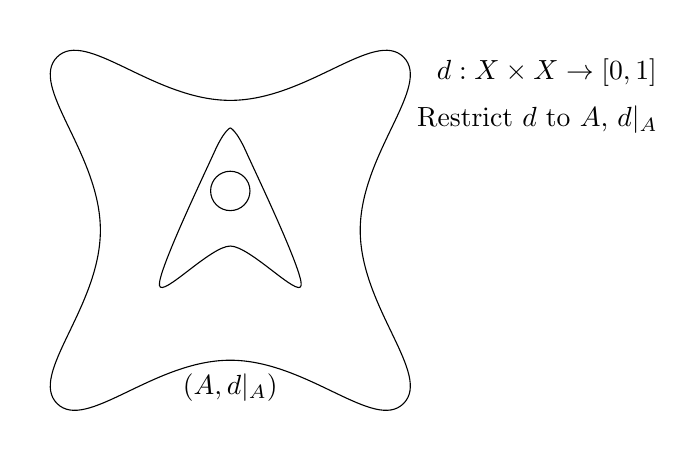
\begin{tikzpicture}[scale=1]
         \draw plot[smooth cycle, tension=0.8, scale=1.1] coordinates {(2,2) (1.5,0) (2,-2) (0,-1.5) (-2,-2) (-1.5,0) (-2,2) (0,1.5)};
         \draw plot[smooth, tension=0.5] coordinates {(0,1.3) (-0.2,1) (-0.9,-0.7) (0,-0.2) (0.9,-0.7) (0.2,1) (0,1.3)};
         \draw (0,0.5) circle [radius=0.25];
         \node[right] at (2.5,2){$d:X\times X\to[0,1]$};
         \node[below] at (0,-1.7){$(A, d|_{A})$};
         \node[below] at (3.9,1.7){Restrict $d$ to $A$, $d|_{A}$};
    \end{tikzpicture}
\end{center}
$d|_{A}$ is way of evaluating $d$ only using points from $A$. It's what we refer to as a restriction.

Take $(\mathbb{R},d)$ and take the subset $[0,1]$. Consider $\Lambda=\{x\in\mathbb{R}:d(x,1)<\frac{1}{2}\}$, consider the set of points $x$ lying in the subspace $[0,1]$ which are within $(1/2)$ of $1$.
\begin{align*}
    \bigg{\{}x\in A:d(x,1)<\frac{1}{2}\bigg{\}}=\bigg{(}\frac{1}{2},1\bigg{]}
\end{align*}

Now $(\mathbb{R}^{2}, d_{2})$ \& consider the subset $S^{1}=\{(x,y)\in\mathbb{R}:(x^{2}+y^{2})=1\}$:

\begin{multicols}{2}
    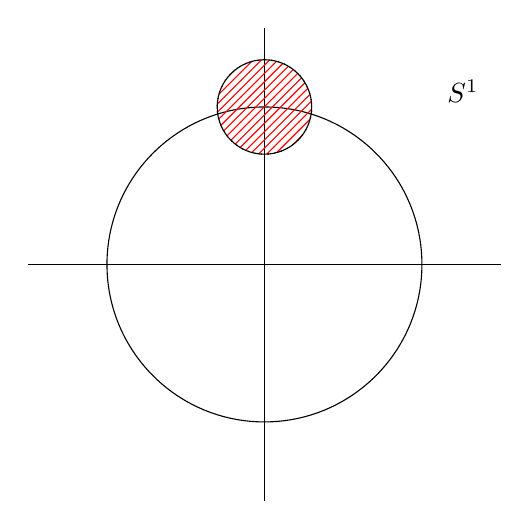
\begin{tikzpicture}[scale=2]
        \draw[-](0,-1.5)--(0,1.5);
        \draw[-](-1.5,0)--(1.5,0);
        \draw[-](0,0) circle [radius=1];
        \draw[-,dotted](0,1) circle [radius=0.3];
        \draw[pattern color=red, pattern=north east lines](0,1) circle [radius=0.3];
        \node[right] at (1.1,1.1){$S^{1}$};
    \end{tikzpicture}

    \begin{tikzpicture}[scale=2]
        \draw[-](0,-1.5)--(0,1.5);
        \draw[-](-1.5,0)--(1.5,0);
        \draw[-](0,0) circle [radius=1];
        \draw[-,dotted](0,1) circle [radius=0.3];
        \node[right] at (1.1,1.1){$S^{1}$};
        \draw[line width=0.1cm, red](0.296605799,0.955) arc [start angle=72.74614688, delta angle=34.5070624, radius=1];
    \end{tikzpicture}
\end{multicols}

If we restrict the area of the small circle to the big circle set or $d|_{\text{Big circle}}$, it becomes the arc shown in the second image. 

%\draw[-](0,0)--(0,1);
%\draw[-](0,0)--(1,0);
\subsection{\& Isometry}
Question: When is $(X,d)$ the `same' as $(X,\hat{d})$? It depends on our definition of `same'. Perhaps when `same' is an Isometry, it is most rigid.
\begin{quote}
    Let $(X,d)$ be a metric space \& let $A\subseteq Y$ where $Y$ is a metric space $(Y,\hat{d})$. We say $X$ is isometric to $A$ if $\exists\psi:X\to A$ which is surjective \& $(\star)\,\hat{d}(\psi(a), \psi(b))=d(a,b)\,\forall a,b\in X$ upshot $\psi(X)$ is a subspace of $(Y,\hat{d})$. We say that $X$ and $Y$ are isometric if $\psi(X)=Y$ and $(\star)$ holds.
\end{quote}
The map $\psi$ is an isometry. For example: $\psi:\mathbb{R}\to\mathbb{C};\,t\mapsto t+0i$. $\mathbb{C}$ is a metric space. The standard metric we can put on it is the Euclidean metric so $(\mathbb{C}, |\cdot|)$. $\psi^{*}:\mathbb{R}\to\mathbb{C}\,;t\mapsto t_{2}$ (maps onto the $y$-axis) is also an isometry. $\mathbb{R}^{2}$ is isometric to $\mathbb{C}$. Why? $\psi:\mathbb{R}\to\mathbb{C};\,(x,y)\mapsto x+iy$. Verify the distance $|(x+iy)-(x'-iy')|=|(x-x')+i(y-y')|=\sqrt{(x-x')^{2}+(y-y')^{2}}=|(x,y)-(x',y')|$. So as metric spaces, these two sets are the same as all the metric cares about is the distance. 

\newpage

\section{The (Basic) Geometry of Metric Spaces}
\subsection{Interior, Exterior and Boundaries}
Note: We can write the sets $(0,1)=\{x\in\mathbb{R}:|x-\frac{1}{2}|<\frac{1}{2}\}$ and $(a,b)=\{x\in\mathbb{R}:|x-\frac{a+b}{2}|<\frac{1}{2}\}$. Consider the open \& closed interval in $\mathbb{R}$: 
\begin{align*}
    (0,1)&=\{x\in\mathbb{R}:0<x<1\} & [0,1]&=\{y\in\mathbb{R}:0\leq y\leq1\}
\end{align*}
Let $(X,d)$ be a metric space. Then for any $x\in X$ and $r\in(a,b)$ the open ball centered at $x$ of radius $r$ which is denoted by $B(x,r)$ is the set $B(x,r)=\{y\in X:d(y,x)\leq r\}$. Analogue of $(a,b)\subset\mathbb{R}$: 
\begin{align*}
    \text{Take }[a,b]&=\{t\in\mathbb{R}:a\leq t\leq b\},\\
    \text{then }[a,b]&=\bigg{\{}t\in\mathbb{R}:d\Big{(}t,\frac{a+b}{2}\Big{)}\leq\frac{b-a}{2}\bigg{\}}.
\end{align*}
let $(X,d)$ be a metric space \& $x\in X$, $r\in(0,\infty)$. The closed ball centered $x$ of radius $r$, $B(x,r)$ is the set: \begin{equation*}\bar{B}(x,r)=\{y\in X:d(y,x)\leq r\}\end{equation*}
But why do we care about $B(x,r)$ \& $\bar{B}(y,s)$? Think about the role that $(a,b)$ plays in analysis; Consider the continuous function $f$ at $x_{0}$;
\begin{quote}
    $f:\mathbb{R}\to\mathbb{R}$ is continuous at $x_{0}\in\mathbb{R}\iff\forall\varepsilon>0,\,\,\exists\delta>0$ such that $|f(x)-f(x_{0})|<\epsilon$ whenever $|x-x_{0}|<\delta$. $-\delta<x-x_{0}<\delta\iff x_{0}-\delta<x<x_{0}+\delta\iff x\in B(x_{0},\delta)$.
\end{quote}
What is the difference geometrically? 
\begin{center}
    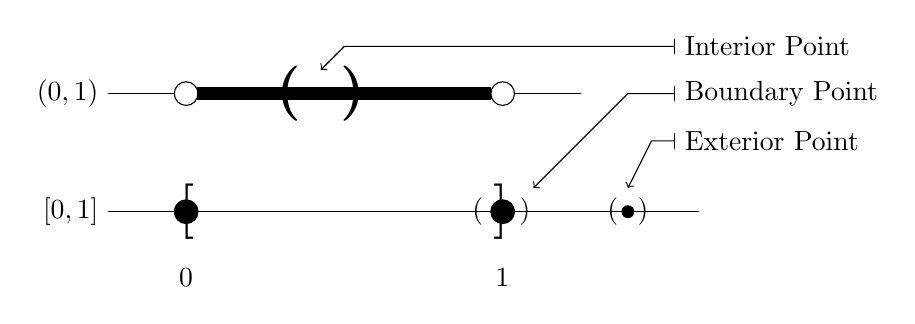
\begin{tikzpicture}[scale=3]
        \draw[-](-1,0.5)--(1,0.5);
        \draw[-](-1,0)--(1.5,0);
        \draw[fill, white] (-0.67,0.5) circle [radius=0.05];
        \draw[fill, white] (0.67,0.5) circle [radius=0.05];
        \draw[fill] (-0.67,0) circle [radius=0.05];
        \draw[fill] (0.67,0) circle [radius=0.05];
        \draw[-] (-0.67,0.5) circle [radius=0.05];
        \draw[-] (0.67,0.5) circle [radius=0.05];
        \node[left, scale=2] at (-0.55,0){[};
        \node[right, scale=2] at (0.55,0){]};
        \draw[fill](-0.62,0.475) rectangle (0.62,0.525);
        \node[below] at (-0.67,-0.2){$0$};
        \node[below] at (0.67,-0.2){$1$};
        \node[right] at (0.7,0){)};
        \node[right] at (0.5,0){(};
        \draw[-, fill] (1.2,0) circle [radius=0.025];
        \node[right] at (1.2,0){)};
        \node[left] at (1.2,0){(};
        \node[right, scale=2] at (-0.1,0.5){\textbf{)}};
        \node[left, scale=2] at (-0.1,0.5){\textbf{(}};
        \node[right] at (1.4,0.7){Interior Point};
        \node[right] at (1.4,0.5){Boundary Point};
        \node[right] at (1.4,0.3){Exterior Point};
        \draw[|->](1.4,0.7)--(0,0.7)--(-0.1,0.6);
        \draw[|->](1.4,0.5)--(1.2,0.5)--(0.8,0.1);
        \draw[|->](1.4,0.3)--(1.3,0.3)--(1.2,0.1);
        \node[left] at (-1,0.5){$(0,1)$};
        \node[left] at (-1,0){$[0,1]$};
    \end{tikzpicture}
\end{center}
\begin{quote}
    After taking a small enough interval around $x$, where $x\in(0,1)$, it always stays inside the set. If we set $x=1$ then for any interval of any length, it hits outside of the set. This is important when defining these points.
\end{quote}
\begin{itemize}
    \item\textbf{Interior Points}: let $A\subset X$. An interior point $y\in X$ of $A$ is an element which $B(y,\varepsilon)\subset A$ for some $\varepsilon>0$
    \subitem We call the set of interior points of $A$, the interior of $A$ \& we denote the set by $A^{o}$.
    \item\textbf{Boundary Points}: The element $y\in X$ is a boundary point of $A\iff$ for any $\varepsilon>0$, $B(y,\varepsilon)\cap A\neq\emptyset$ and $B(y,\varepsilon)\cap(A^{c})\neq\emptyset$. The boundary of $A$, denoted $\partial A$, is the set of all boundary points of $A$.
    \item\textbf{Exterior Points}: An element $y$ of $X$ is an exterior point of $A\iff\exists\varepsilon>0$ for which $B(y,\varepsilon)\subset A^{c}$. The exterior of $A$ is the set of all exterior points of $A$, denoted $A^{e}$.
\end{itemize}

\begin{multicols}{2}
\begin{itemize}
\item[Example:] Calculate $A^{2}$, $\partial A$ and $A^{c}$ 

where $A=(0,1]\subset\mathbb{R}$:
\end{itemize}
\begin{align*}
    A^{e}&=(-\infty,0)\cup(1,\infty)\\
    A^{o}&=(0,1)\\
    \partial A&=\{0,1\}
\end{align*}

Facts:
\begin{align*}
X=\underbrace{\partial A\sqcup A^{e}\sqcup A^{o}}_{\text{Disjoint Union}}
    \begin{cases}
        \partial A\cup A^{e}\cup A^{o}=X\\
        \partial A\cap A^{o}=\emptyset\\
        \partial A\cap A^{e}=\emptyset\\
        A^{o}\cap A^{e}=\emptyset
    \end{cases}
\end{align*}
\end{multicols}
$(\mathbb{R},d)$ where $d(x,y)=|x-y|$. Take $x\in(0,1)$ so $0<x<1$. 
\begin{center}
    \begin{tikzpicture}[scale=2, xscale=2]
        \draw[-](-1,0)--(1,0);
        \node[] at (-1,0){(};
        \node[] at (1,0){)};
        \node[below] at (-1,-0.1){0};
        \node[below] at (1,-0.1){1};
        \draw[-](-0.3,-0.1)--(-0.3,0.1);
        \node[below] at (-0.3,-0.1){$x$};
        \node[left] at (-0.4,0){(};
        \node[right] at (-0.2,0){)};
        \node[above] at (-0.3,0.1){$B$};
        \draw[<->](-1,-0.4)--(-0.3,-0.4);
        \draw[<->](-0.3,-0.4)--(1,-0.4);
        \node[below] at (-0.6,-0.4){$\varepsilon$};
        \node[below] at (0.4,-0.4){$\varepsilon'$};
    \end{tikzpicture}
\end{center}
Let $\varepsilon=x-0$ and $\varepsilon'=1-x$, let $\varepsilon^{*}=\min\{\varepsilon,\varepsilon'\}$. Consider $B(x,\frac{\varepsilon^{*}}{2})$. Then $B(x,\frac{\varepsilon^{*}}{2})\subset A$. \textbf{Why?} If $y\in B(x,\frac{\varepsilon^{*}}{2})$ then $|y-x|<\frac{\varepsilon^{*}}{2}$. So $-\frac{\varepsilon^{*}}{2}<y-x<\frac{\varepsilon^{*}}{2}$ and $0<x-\varepsilon^{*}<x-\frac{\varepsilon^{*}}{2}<y<x+\frac{\varepsilon^{*}}{2}$. But \textbf{Why} is $0<x-\frac{\varepsilon^{*}}{2}$? Because $\varepsilon=x-0$ and $\varepsilon^{*}=\min\{\varepsilon,\varepsilon'\}$ so $\frac{\varepsilon^{*}}{2}<\varepsilon^{*}\leq\varepsilon$.

Thus far $(0,1)\subset(0,1]^{o}$. What about $x<0$? Not possible. \textbf{Why?} See the definition of the interior point. Similarly, $x>1$ cannot be an interior point. Any interior point is an element of the set. So $A^{o}\subseteq(0,1]$. What about $1\in A^{o}$? No. Take $\varepsilon>0$ and $B(1,\varepsilon)$ Then  this contains a point $y>1$. Then this contains a point $y>1$ and $y\notin A$. Thus $A^{o}=(0,1)$. 

$\partial A=\{0,1\}$. Claim $0$ and $1$ are boundary points. \textbf{Why?} Take any $\varepsilon>0$. Consider $B(0,\varepsilon)=B(-\varepsilon,\varepsilon)$ then $B(0,\varepsilon)\cap A\neq\emptyset$. \textbf{Why?} Take $\delta>0$ such that $\delta>\varepsilon$ and $\delta>1$. Further as $\exists y\in B(0,\varepsilon)$ for which $y<0$ the intersection of $B(0,\varepsilon)\cap A^{c}\neq\emptyset$. Similar Argument for 1. 
\begin{itemize}
    \item[Fact:] If $y\in\partial B$ then $y$ might be an element of $B$, but it might not. 
\end{itemize}
Are there any other boundary points? As $A^{o}\cap\partial A=\emptyset$ then no point in $(0,1)$ can be a boundary point. What about $y<0$ or $y>1$? No, let $y>1$ then $\exists\varepsilon>0$ such that $y=1+\varepsilon$. Take the ball $B(y,\frac{\varepsilon}{10})$ then $B(y,\frac{\varepsilon}{10})\subset A^{c}$. 
\begin{itemize}
    \item[Fact:] $\partial\emptyset=\emptyset$ and $\partial X=\emptyset$.
\end{itemize}
\begin{align*}
    (0,1)&:\text{Open} & [0,1]&:\text{Closed} & (0,1]&:\text{Half-Closed}
\end{align*}
So let $(X,d)$ be a metric space.
\begin{itemize}
    \item A subset $A$ of $X$ is open $\iff A\cap\partial A=\emptyset$.
    \item A subset $F$ of $X$ is closed $\iff\partial F\subseteq F$. 
\end{itemize}
$X$ is Clopen. $\partial X=\emptyset$ so $\partial X\cap X=\emptyset\cap X=\emptyset$ (Open) and $\emptyset=\partial X\subseteq X$ (Closed).
\begin{quote}
    Example: $(\mathbb{R},d)$. $A=(0,1)\cup(1,2)$. As $\partial A=\{0,1,2\}$ we see that $A\cap\partial A=\emptyset$ so $A$ is open. Further $\partial A\nsubseteq A$ so not closed. Now consider $A$ as a subspace $(A,d)$, $\partial A=\emptyset$, $A^{o}=A\implies A^{e}=\emptyset$. Now $(0,1)\subseteq(0,1)\cup(1,2)$ is clopen as $\partial(0,1)=\emptyset\implies\partial(0,1)\cap(0,1)=\emptyset$ (Open) and $\partial(0,1)=\emptyset\subseteq(0,1)$ thus, $(0,1)$ is closed. 
\end{quote}

\subsection{Visualisation of Interior, Exterior and Boundary Points}
Visualisation of $A^{o}$, $A^{e}$, $\partial A$ in $\mathbb{R}^{2}$
\begin{center}
    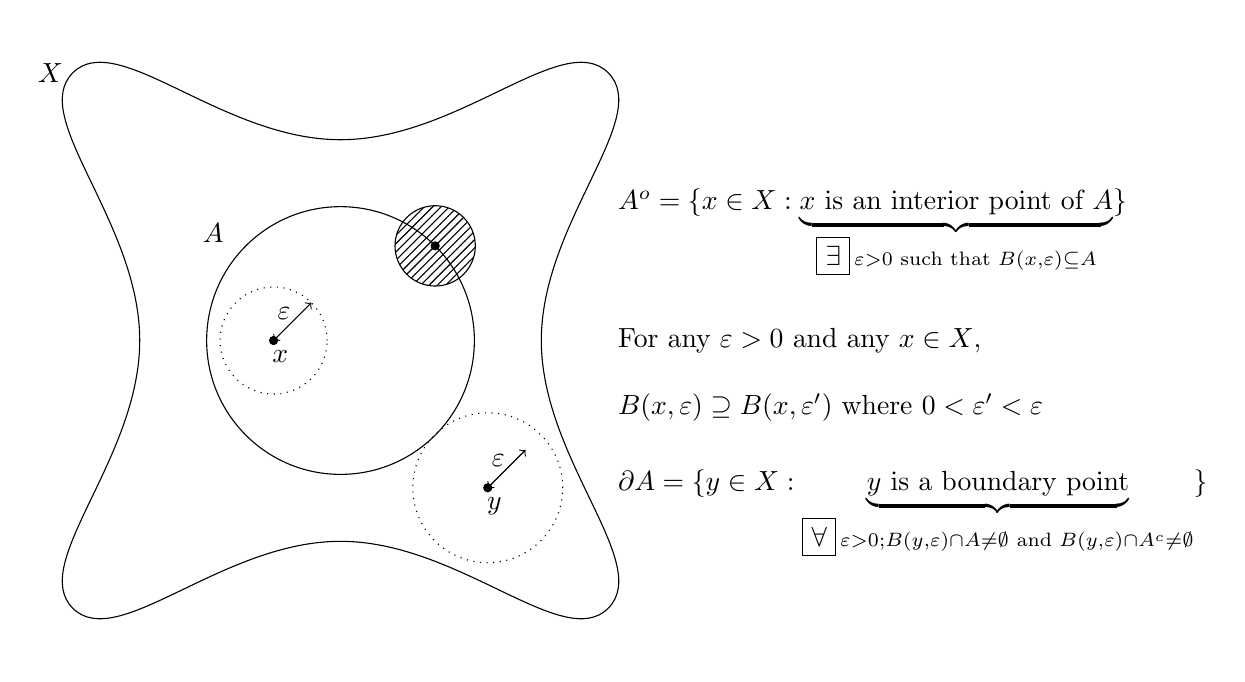
\begin{tikzpicture}[scale=1.7]
        \draw plot[smooth cycle, tension=0.8] coordinates {(2,2) (1.5,0) (2,-2) (0,-1.5) (-2,-2) (-1.5,0) (-2,2) (0,1.5)};
        \node[left] at (-2,2){$X$};
        \draw[-, radius=1](0,0) circle;
        \node[left] at (-0.8,0.8){$A$};
        \draw[dotted, radius=0.4](-0.5,0) circle;
        \draw[fill, radius=0.03](-0.5,0) circle;
        \node[below] at (-0.45,0){$x$};
        \draw[<->](-0.5,0)--(-0.2171572875, 0.2828427125);
        \node[left] at (-0.3, 0.2){$\varepsilon$};
        \draw[dotted, radius=0.56](1.1,-1.1) circle;
        \draw[fill, radius=0.03](1.1,-1.1) circle;
        \node[below] at (1.15,-1.1){$y$};
        \draw[<->](1.1,-1.1)--(1.382842712,-0.8171572875);
        \node[left] at (1.3,-0.9){$\varepsilon$};
        \draw[-, radius=0.3, pattern=north east lines](0.7071067812, 0.7071067812) circle;
        \draw[fill, radius=0.03](0.7071067812, 0.7071067812) circle;
        \node[right] at (2,0){For any $\varepsilon>0$ and any $x\in X$,};
        \node[right] at (2,-0.5){$B(x,\varepsilon)\supseteq B(x,\varepsilon')$ where $0<\varepsilon'<\varepsilon$};
        \node[right] at (2,0.8){$A^{o}=\{x\in X:\underbrace{\text{$x$ is an interior point of $A$}}_{\boxed{\exists}\,\varepsilon>0\text{ such that }B(x,\varepsilon)\subseteq A}\}$};
        \node[right] at (2,-1.3){$\partial A=\{y\in X:\underbrace{\text{$y$ is a boundary point}}_{\boxed{\forall}\,\varepsilon>0;B(y,\varepsilon)\cap A\neq\emptyset\text{ and }B(y,\varepsilon)\cap A^{c}\neq\emptyset}\}$};
        
    \end{tikzpicture}
\end{center}

Open: $A\cap\partial A=\emptyset$, Closed: $\partial A\subseteq A$ and $\partial\emptyset=\emptyset$ and $\partial X=\emptyset$ \textbf{Fact:} If $A\subseteq X$ then $A^{o}\sqcup A^{e}\sqcup\partial A=X$. \textbf{Fact:} If $A\subseteq X$ is open $\iff A^{c}$ is closed. Proof:
\begin{quote}
    Let's assume that $A\subseteq X$ is open. If $A=\emptyset$ then $A^{c}=X$ and $X$ is closed. So we can assume that $A\neq\emptyset$. By definition, $\partial A\cap A=\emptyset$ (open), so $\partial A\subseteq A^{c}$. But $\partial A=\partial A^{c}$. As $\partial(A^{c})=\{y\in X:\text{$y$ is a boundary point of $A^{c}$}\}$. $y$ is such that $\forall\varepsilon>0$, $B(y, \varepsilon)\cap A^{c}\neq\emptyset$ and $B(y,\varepsilon)\cap(A^{c})^{c}\neq\emptyset$. Thus $A^{c}$ is closed. Assume that $A$ is closed. By definition, $\partial A\subseteq A$ so $\partial A\cap A^{c}=\emptyset$ and hence $\partial A^{c}\cap A^{c}=\emptyset$ and hence $A^{c}$ is open. Thus; $A$ is open $\iff A^{c}$ is closed.
\end{quote}

\subsection{Topology of a Metric Space}
The topology of $(X,d)$: So, the topology of a metric space, $T_{d}$ is the collection of all open subsets of $(X,d)$. Note: $T_{d}\subseteq\mathcal{P}(X)=\text{ (The power set of $X$)}$ and $T_{d}\neq\emptyset$ as $\emptyset$, $X\in T_{d}$. (More on topology later).

Think about:
\begin{center}
\begin{tikzpicture}[scale=3]
    \draw[-](-2,0)--(2,0);
    \node[right, scale=3] at (-2,0){(};
    \node[left, scale=3] at (2,0){)};
    \node[below] at (-1.8,-0.2){$a$};
    \node[below] at (1.8,-0.2){$b$};
    \draw[-](0,-0.3)--(0,0.3);
    \draw[-](1,-0.1)--(1,0.1);
    \node[above] at (0,0.3){$\frac{a+b}{2}$};
    \node[below] at (1,-0.1){$x$};
    \draw[<->](0,0.1)--(1,0.1);
    \draw[<->](1,0.1)--(1.8,0.1);
    \node[above] at (0.5,0.1){$\varepsilon'$};
    \node[above] at (1.4,0.1){$\varepsilon$};
\end{tikzpicture}
\end{center}
$\varepsilon+\varepsilon'=\frac{b-a}{2}$. One of $\varepsilon$ and $\varepsilon'$ are minimal, so without loss of generality assume $\varepsilon=\min\{\varepsilon,\varepsilon'\}$. The graph above is used to motivate $B(x,\varepsilon)$. So $B(x,\varepsilon^{*})\subseteq(a,b)$ where $\varepsilon^{*}=\varepsilon/2$.
\begin{itemize}
    \item[Fact:] If $A\subseteq X$ is open, then every point of $A$ is an interior point of $A$. Equivalently, For any $x\in A$, $\exists\varepsilon$ such that $A$ (open) $\iff\varepsilon=\varepsilon(x)>0$ such that $B(x,\varepsilon)\subseteq A$. $A$ is open $\sim\partial A\cap A=\emptyset$ by definition.
\end{itemize}
\begin{enumerate}
    \item $A=\emptyset$ as $\emptyset$ is open.
    \item $A\neq\emptyset$. There must be at least one $\varepsilon>0$ such that $B(x,\varepsilon)\subseteq A$ or $B(x,\varepsilon)\subseteq A^{c}$ for any $x\in A$. But $x\in A$ and $x\in B(x,\varepsilon)$, so $B(x,\varepsilon)\subseteq A^{c}$ is impossible! Therefore $B(x,\varepsilon)\subseteq A$.
\end{enumerate}

Assume that $\forall x\in A$, $\exists \varepsilon>0$ such that $B(x,\varepsilon)\subseteq A$. Thus $x\notin\partial A$. For $x\in\partial A$ we would need $B(x,\varepsilon)\cap A^{c}\neq\emptyset$ and this isn't possible.
\begin{multicols}{3}
    \begin{itemize}
    \item $A_{\text{open}}\iff A^{c}_{\text{closed}}$
    \item $A_{\text{open}}\iff\partial A\cap A=\emptyset$
    \item $A_{\text{open}}\iff\forall x\in A,\,\exists\varepsilon=\varepsilon(x)>0$ such that $B(x\varepsilon)\subseteq A$.
\end{itemize}
\end{multicols}

$T_{d}$ is the collection of all open subsets of $(X,d)$; $\{\emptyset, X\}\subseteq T_{d}$. 
\begin{itemize}
    \item[Fact:] For any $x\in X$ and any $\varepsilon>0$, $B(x,\varepsilon)\in T_{d}$ (Open ball is open).
\end{itemize}

Proof:
\begin{multicols}{2}
\begin{center}
    \begin{tikzpicture}[scale=2.5]
        \draw[dotted, radius=1](0,0) circle;
        \draw[fill, radius=0.04](0,0) circle;
        \draw[<->](0,0)--(0.70710678118,0.70710678118);
        \node[below] at (0,0){$x$};
        \node[below] at (0.4,0.4){$\varepsilon$};
        \draw[fill, radius=0.03](0,0.5) circle;
        \node[left] at (0,0.5){$y$};
        \draw[dotted, radius=0.2](0,0.5) circle;
        \draw[-](0,0)--(0,1.3);
        \node[left, scale=2.5] at (0.1,0.25){$\{$};
        \node[left] at (-0.15,0.25){$\varepsilon'$};
    \end{tikzpicture}
\end{center}

Take $y\in B(x,\varepsilon)$. If $y=x$ we are done. Consider $B(y,\varepsilon)=B(x,\varepsilon)\subseteq B(x,\varepsilon)$.

Assume $y\neq x$. Then $d(x,y)=\Delta>0$ and $0<\Delta<\varepsilon$. So we set $\varepsilon'=\min\{\Delta,\varepsilon-\Delta\}$ and $\varepsilon^{*}=\varepsilon'/2$. Claim: Ball $B(y,\varepsilon^{*})\subseteq B(x,\varepsilon)$. We want to show that $d(x,z)<\varepsilon$ for any $z\in B(y,\varepsilon^{*})$. It would follow that $z\in B(x,\varepsilon)$ and $B(y,\varepsilon^{*})\subseteq B(x,\varepsilon)$. So
\begin{align*}
    d(x,z)&\leq d(x,y)+d(y,z)\\
    &\leq\Delta+\varepsilon^{*}\\
    &\leq\Delta+\min\{\Delta,\varepsilon-\Delta\}/2\\
    &\leq\Delta+\frac{\varepsilon-\Delta}{2}\\
    &\boxed{<}\Delta+\varepsilon-\Delta\\
    &=\varepsilon.
\end{align*}
Thus $z\in B(x,\varepsilon)\forall z\in B(y,\varepsilon^{*})$ and therefore $B(y,\varepsilon^{*})\subseteq B(x,\varepsilon)$.
Fact: If $A\in T_{d}$ \& $A\neq\emptyset$ then $A$ is a union of open balls
\end{multicols}
We are given $A\neq\emptyset$ and $A_{\text{open}}$. 

Take an $x\in A$, we know $\exists\varepsilon=\varepsilon(x)>0$ such that $B(x,\varepsilon(x))\subseteq A$ then $A=\bigcup_{x\in A}B(x,\varepsilon(x))$. 

Why? $A\subseteq\cup B(x,\varepsilon(x))$ as $x\in B(x,\varepsilon(x))$. Further $\cup B(x,\varepsilon(x))\subseteq A$ as $B(x,\varepsilon(x))\subseteq A$. 
\begin{quote}
    \boxed{\text{$A=B$, can be proven showing $A\subseteq B$ and $B\subseteq A$}}
\end{quote}

Question: Can we now determine key properties of $T_{d}$? Yes!

Fact: Take any collection of open sets $\Lambda\in T_{d}$ then the union of the sets in $\Lambda$ is open. For any $\Lambda\in T_{d}$, $\bigcup_{\Omega\in\Lambda}\Omega\in T_{d}$.

Take $x\in\bigcup_{\Omega\in\Lambda}\Omega$, we know $\exists\Omega(x)\ni x$ \& $\Omega(x)$ is open $\implies\exists\varepsilon>0$ such that $B(x,\varepsilon)\subseteq\Omega(x)\implies B(x,\varepsilon)\subseteq\bigcup_{\Omega\in\Lambda}\Omega$.

Question: Unions work, but will intersections work? No! Finite intersections work, but infinite intersections do not. 
\begin{quote}
    Example: Take $(\mathbb{R}, d)$ and consider $I_{n}=(-\frac{1}{n},\frac{1}{n})$. then $\bigcap_{n=1}^{\infty}I_{n}=\{0\}$ and $\{0\}\notin T_{d}$. 
\end{quote}
Visual Proof:
\begin{center}
\begin{tikzpicture}[scale=2, xscale=2]
    \draw[<->](-1.5,0)--(1.5,0);%All the horizontal lines
    \draw[<->](-1.5,-0.5)--(1.5,-0.5);
    \draw[<->](-1.5,-1)--(1.5,-1);
    \draw[<->](-1.5,-1.5)--(1.5,-1.5);
    % - Brackets
    \node[scale=2] at (1,0){)};
    \node[scale=2] at (-1,0){(};
    \node[scale=2] at (0.5,-0.5){)};
    \node[scale=2] at (-0.5,-0.5){(};
    \node[scale=2] at (0.3333333333333333,-1){)};
    \node[scale=2] at (-0.3333333333333333,-1){(};
    \node[scale=2] at (0.25,-1.5){)};
    \node[scale=2] at (-0.25,-1.5){(};
    % - Set Labels I_n
    \node[left, scale=1] at (-1.5,0){$I_{1}:$};
    \node[left, scale=1] at (-1.5,-0.5){$I_{2}:$};
    \node[left, scale=1] at (-1.5,-1){$I_{3}:$};
    \node[left, scale=1] at (-1.5,-1.5){$I_{4}:$};
    % - Real line labels
    \node[right, scale=1] at (1.5,0){$\mathbb{R}$};
    \node[right, scale=1] at (1.5,-0.5){$\mathbb{R}$};
    \node[right, scale=1] at (1.5,-1){$\mathbb{R}$};
    \node[right, scale=1] at (1.5,-1.5){$\mathbb{R}$};
    % - Dotted lines
    \draw[dotted](-1,0)--(-1,-1.9);%dotted for 1
    \draw[dotted](1,0)--(1,-1.9);
    \draw[dotted](-0.5,-0.5)--(-0.5,-2);%dotted for 1/2
    \draw[dotted](0.5,-0.5)--(0.5,-2);
    \draw[dotted](-0.333333333,-1)--(-0.333333333,-2.2);%dotted for 1/3
    \draw[dotted](0.333333333,-1)--(0.333333333,-2.2);
    \draw[dotted](-0.25,-1.5)--(-0.25,-2.45);%dotted for 1/4
    \draw[dotted](0.25,-1.5)--(0.25,-2.45);
    \draw[dashed](0,0.4)--(0,-2);%dotted for 0
    % - Number labels for dotted lines
    \node[below] at (-1,-1.9){$-1$};
    \node[below] at (1,-1.9){$1$};
    \node[below] at (-0.55,-2){$-\frac{1}{2}$};
    \node[below] at (0.5,-2){$\frac{1}{2}$};
    \node[below] at (-0.4,-2.2){$-\frac{1}{3}$};
    \node[below] at (0.333333333,-2.2){$\frac{1}{3}$};
    \node[below] at (-0.3,-2.45){$-\frac{1}{4}$};
    \node[below] at (0.25,-2.45){$\frac{1}{4}$};
    \node[below] at (0,-2){$0$};
    % - Extra bits!
    \draw[->](-2,-0.4)--(-2,-1.2);
    \node[above] at (-2,-0.4){$n$};
    \node[below] at (-2,-1.2){$\infty$};
    \draw[->](-0.8,0.5)--(-0.01,0.5);
    \draw[->](0.8,0.5)--(0.01,0.5);
    \node[left] at (-0.8,0.5){$-\frac{1}{n}$};
    \node[right] at (0.8,0.5){$\frac{1}{n}$};
\end{tikzpicture}
\end{center}

Fact: Take any finite collection of open sets $\Omega_{1}$, $\dots$, $\Omega_{n}\in T_{d}$. Then $\bigcap_{i=1}^{N}\Omega_{i}$ is open. Why? 

If $\bigcap_{i=1}^{N}\Omega_{i}=\emptyset$ then we're done as $\emptyset$ is open.

Assume $\bigcap_{i=1}^{N}\Omega_{i}\neq\emptyset$. Take any $x\in\bigcap_{i=1}^{N}\Omega_{i}$, then $\exists\varepsilon_{i}>0$ for which $B(x,\varepsilon_{i})\subseteq\Omega_{i}$ and take $\varepsilon=\min\{\varepsilon_{1}, \varepsilon_{2},\dots,\varepsilon_{n}\}$ then $B(x,\varepsilon)\subseteq B(x,\varepsilon_{1})\subseteq\Omega_{i}$ for $i=1,2,\dots,N$ and thus $B(x,\varepsilon)\subseteq\bigcap_{i=1}^{N}\Omega_{i}$.

\subsection{Rules of Topology}
Quick recap:
\begin{multicols}{2}
    \begin{itemize}
    \item We've defined open \& closed via open balls (Rather than via $\partial A\cap A=\emptyset$ (open) \& $\partial A=A$ (closed))
    \item Derived the rules for working with the collection of all open sets, $T_{d}$: the set of all open subsets of $X$, the topology induced by the metric $d$.
\end{itemize}
\end{multicols}

$\Omega\subseteq X$, is an element of $T_{d}\iff\partial\Omega\cap\Omega=\emptyset\iff$ for any $x\in\Omega$, $\exists\varepsilon=\varepsilon(x)>0$ such that $B(x,\varepsilon)\subseteq\Omega$.

Any open set is either empty or is the union of open balls. Let $(X,d)$ be a metric space \& $T_{d}$ be the topology induced by $d$,
\begin{enumerate}[label=\textbf{T\arabic*)}]
    \item $\emptyset$, $X\in T_{d}$ 
    \item $T_{d}$ is closed under arbitrary unions
    \item $T_{d}$ is closed under \underline{finite} unions.\footnote{Subtle point on \textbf{(T3)}: It's possible that an infinite collection of open sets \underline{might} have an open intersection. It just is not certain in general.}
\end{enumerate}

Alternative:
\begin{enumerate}[start=2, resume*]
    \item For any collection of open sets $\Lambda\subseteq T_{d}$, $\bigcup_{\Omega\in\Lambda}\Omega\in T_{d}$
    \item For any \boxed{\text{finite}} collection of open sets $(\Omega_{1}, \Omega_{2}, \dots, \Omega_{N})$, $\bigcap_{i=1}^{N}\Omega_{i}\in T_{d}$.
\end{enumerate}



Note: $\{a\}\subseteq X$ then $\{a\}$ is closed (closed: $\partial A\subseteq A$ or $A^{c}\in T_{d}$) if $X=\{a\}$ then $\{a\}$ is closed and open. So if $X=\{a\}$ then $X$ has at least 2 elements inside. Well, $\partial\{a\}=\{a\}$ so $\partial A\subseteq A$. Why? Take any $\varepsilon>0$, consider $B(a,\varepsilon)$ then $B(a,\varepsilon)\cap\{a\}\neq\emptyset$. 

If $X=\{a,b\}$, $d:X\to[0,\infty)$ and $d(a,b)=\gamma>0$. Then
\begin{align*}
    B\bigg{(}a,\frac{\gamma}{2}\bigg{)}
    &=\bigg{\{}x\in X\,\bigg{|}\,d(a,x)<\frac{\gamma}{2}\bigg{\}}=\{a\} 
    & B\bigg{(}a,\frac{\gamma}{N}\bigg{)}
    &=\bigg{\{}x\in X\,\bigg{|}\,d(a,x)<\frac{\gamma}{N}\bigg{\}}=\{a\}
\end{align*}
$\mathbb{Q}$-$p$-adic Metric where $p$ is a prime number (this is the future):
\begin{align*}
    d(q,q')\in\{p^{-n}\,|\,n\in\mathbb{Z}\}
\end{align*}
\newpage
\begin{itemize}
    \item[Question:] What happens to T2) \& T3) if we replace open with closed?
\end{itemize}


\textbf{T2)}? Take a collection of closed sets. Let $\mathcal{F}$ be an arbitrary collection of closed sets.
\begin{align*}
    \forall F\in\mathcal{F},\, F^{c}\in T_{d}&\implies\bigcup(F^{c})\in T_{d}\,\textbf{(T2)}\\
    &\implies\bigcap(F)\text{ is closed}.
\end{align*}


De Morgan's Laws:
\begin{align*}
    \bigg{(}\bigcap F\bigg{)}^{c}=\bigcup F^{c}\in T_{d}\implies\bigcap F\text{ is closed.}
\end{align*}
Similarly:
\begin{align*}
    \bigg{(}\underbrace{\bigcap^{N}_{i=1} F_{i}}_{\text{closed}}\bigg{)}^{c}=\bigcap^{N}_{i=1}\underbrace{F^{c}}_{\text{open}}\in T_{d}
\end{align*}
Thus:
\begin{itemize}
    \item[\textbf{F2)}] The union of any finite collection of closed sets is closed.
    \item[\textbf{F3)}] The intersection of any collection of closed sets is closed.
\end{itemize}


Back to $\mathbb{R}^{2}$:
\begin{multicols}{3}
    \begin{itemize}
    \item[$d_{1}$:]
        \begin{center}
            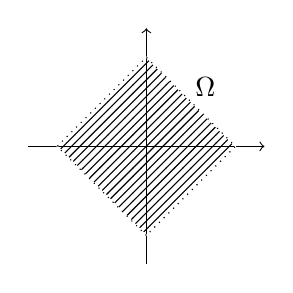
\begin{tikzpicture}
                \draw[->](-1.5,0)--(1.5,0);
                \draw[->](0,-1.5)--(0,1.5);
                \draw[color=white, fill, rotate=45, pattern=north east lines](-0.8,-0.8) rectangle (0.8,0.8);
                \draw[dotted, rotate=45](-0.8,-0.8) rectangle (0.8,0.8);
                \node[right] at (0.5,0.75){$\Omega$};
            \end{tikzpicture}
        \end{center}

    \item[$d_{2}$:]
        \begin{center}
            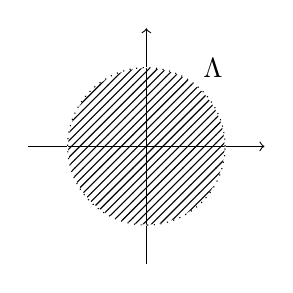
\begin{tikzpicture}
                \draw[->](-1.5,0)--(1.5,0);
                \draw[->](0,-1.5)--(0,1.5);
                \draw[color=white, fill, radius=1, pattern=north east lines](0,0) circle;
                \draw[dotted, radius=1](0,0) circle;
                \node[right] at (0.6,1){$\Lambda$};
            \end{tikzpicture}
        \end{center}

    \item[$d_{\infty}$:]
        \begin{center}
            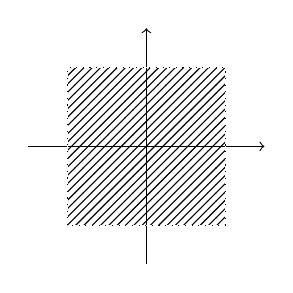
\begin{tikzpicture}
                \draw[->](-1.5,0)--(1.5,0);
                \draw[->](0,-1.5)--(0,1.5);
                \draw[color=white, fill, pattern=north east lines, pattern color=black](-1,-1)--(1,-1)--(1,1)--(-1,1)--(-1,-1);
                \draw[dotted](-1,-1) rectangle (1,1);
            \end{tikzpicture}
        \end{center}
    \end{itemize}
    
\end{multicols}
What about $T_{1}$, $T_{d_{2}}$ \& $T_{d_{3}}$? They're all the same! Why? 

Work in $(\mathbb{R}^{2}, d_{2})$ \& consider $\Omega$. More of the 'same'? 

\begin{center}
    \begin{tikzpicture}[scale=3]
        \draw[->](-1.2,0)--(1.2,0);
        \draw[->](0,-1.1)--(0,1.2);
        \draw[dotted, rotate=45](-0.7071067812,-0.7071067812) rectangle (0.7071067812,0.7071067812);
        \draw[radius=0.03, fill](-0.2, 0.5) circle;
        \draw[-](-0.2, 0.5)--(-0.35,0.65);
        \draw[-](-0.2, 0.5)--(0.65,-0.35);
        \draw[-](-0.2, 0.5)--(-0.85,-0.15);
        \draw[-](-0.2, 0.5)--(0.15,0.85);
        \draw[->](-1,0.6) to [bend right=45] (-0.3,0.57);
        \node[above] at (-1,0.6){$\varepsilon>\varepsilon^{*}=\frac{\varepsilon}{2}$};
        \node[above, scale=0.8] at (-1.1,0){$(-1,0)$};
        \node[right, scale=0.8] at (0,1){$(0,1)$};
        \node[above, scale=0.8] at (1.1,0){$(1,0)$};
        \node[right, scale=0.8] at (0,-1){$(0,-1)$};
        \node[right] at (0.6,0.7){\text{So $\Omega\in T_{d_{2}}$}};
        \draw[->](0.85,0.65) to [bend left=45] (0.5,0.5);
        \node[below] at (-0.2,0.47){$x$};
        \draw[dashed, radius=0.2](-0.2, 0.5) circle;
    \end{tikzpicture}
\end{center}

No matter where the point $x$ is placed, by choosing the shortest distance from the point to the boundary and setting that to $\varepsilon$, we can always construct an open ball $B(x,\varepsilon)$ that is within the set $\Omega$. So $\Omega\in T_{d_{2}}\implies\Omega$ is open!

\newpage
What about $\Lambda$ in $(\mathbb{R}^{2}, d_{1})$?
\begin{center}
    \begin{tikzpicture}[scale=3]
        \draw[->](-1.2,0)--(1.2,0);
        \draw[->](0,-1.1)--(0,1.2);
        \draw[dotted, radius=1](0,0) circle;
        \node[diamond, draw, minimum width = 3cm, minimum height = 3cm, dashed] at (0,0){\empty};
        \draw[fill, radius=0.03](0,0) circle;
        \node[diamond, draw, minimum width = 0.7cm, minimum height = 0.7cm, dashed] at (0.3,-0.4){\empty};
        \draw[fill, radius=0.03](0.3,-0.4) circle;
        \node[diamond, draw, minimum width = 0.3cm, minimum height = 0.3cm, dashed] at (0.5,0.5){\empty};
        \draw[fill, radius=0.03](0.5,0.5) circle;
        \node[diamond, draw, minimum width = 0.7cm, minimum height = 0.7cm, dashed] at (0.6,-0.2){\empty};
        \draw[fill, radius=0.03](0.6,-0.2) circle;
    \end{tikzpicture}
\end{center}
It's the same argument! $\{(x,y)\,|\,x^{2}+y^{2}\leq1\}=\Lambda$ is not an open ball in $(\mathbb{R}^{2},d_{1})$ but it is an open set.

Let $d$ \& $d^{*}$ be metrics on $X$. Then $(X,d)$ \& $(X,d^{*})$ are equivalent $\iff T_{d}=T_{d^{*}}$.

Let $X$ be a set \& $d$, $d^{*}$ be metrics on $X$ such that $\exists\lambda>0$ for which $\frac{1}{\lambda}d(x,y)\leq d^{*}(x,y)\leq\lambda d(x,y)$. Then $T_{d}=T_{d^{*}}$.
\begin{itemize}
    \item[Goal:] Take a set which is not closed and ``make" it closed by adding as few points as possible.
\end{itemize}
Its maximum and its minimum on the interval $f:[a,b]\to\mathbb{R}$ where $f$ is continuous.

\begin{center}
    \begin{tikzpicture}
        \draw[->](-0.1,0)--(7.5,0);
        \draw[->](0,-0.5)--(0,3);
        \draw[-](1.5,-1)--(1.5,1.8) .. controls (1.6,3) and (2.8,3) .. (2.85,1.8)--(2.85,1.8) .. controls (2.9,-1) and (3.8,-1) .. (4.1,-0.9)--(4.1,-0.9) .. controls (4.6,-0.7) and (4.4,-0.1) .. (4.6,-0.1)--(4.6,-0.1) parabola (4.7,-0.2)--(4.7,-0.2) .. controls (4.8,-0.39) and (4.9,-0.2) .. (5,1)--(5,1) .. controls (5.2,3) and (6.8,3) .. (7,1)--(7,1)--(7,-1);
        \node[below] at (1.5,-1) {$a$};
        \node[below] at (7,-1) {$b$};
    \end{tikzpicture}
\end{center}
\begin{itemize}
    \item[Idea:] Add the boundary\footnote{Nothing less works and any more is too much!} to the set.
\end{itemize}
Let $(X,d)$ be a metric space \& $A\subseteq X$. The closure of $A$, denoted by $\overline{A}$, is defined to be
\begin{align*}
    \overline{A}=A\cup\partial A
\end{align*}
``Fact"\footnote{The proof for this so-called Fact comes later.}: There is no superset of $A$, $F$ such that $A\subseteq F\subset\overline{A}\,\,(F\neq\overline{A})$.
\begin{itemize}
    \item[Facts:] 
    \subitem $A\subset\overline{A}=A\cup\partial A$ ($\overline{A}$ is a superset of $A$)
    \subitem $\overline{A}$ is closed. ($\star$)
\end{itemize}
Proof of ($\star$): Show that $(\overline{A})^{c}$ is open:

Consider $(\overline{A})^{c}=\emptyset$ then we're done as $\emptyset$ is open. Now assume $(\overline{A})^{c}\neq\emptyset$. To show $(\overline{A})^{c}$ is open we need to show that for any $x\in(\overline{A})^{c}$, $\exists B(x,\varepsilon)\subseteq(\overline{A})^{c}$. Take $x\in(\overline{A})^{c}$. Thus $x\notin A$ \& $X\notin\partial A$ ($\overline{A}=A\cup\partial A$). As $x\notin\partial A$ then $\exists\varepsilon>0$ such that $B(x,\varepsilon)\subseteq A$ or $B(x,\varepsilon)\subseteq A^{c}$. So $B(x,\varepsilon)\subseteq A^{c}$

\begin{multicols}{2}
\begin{center}
    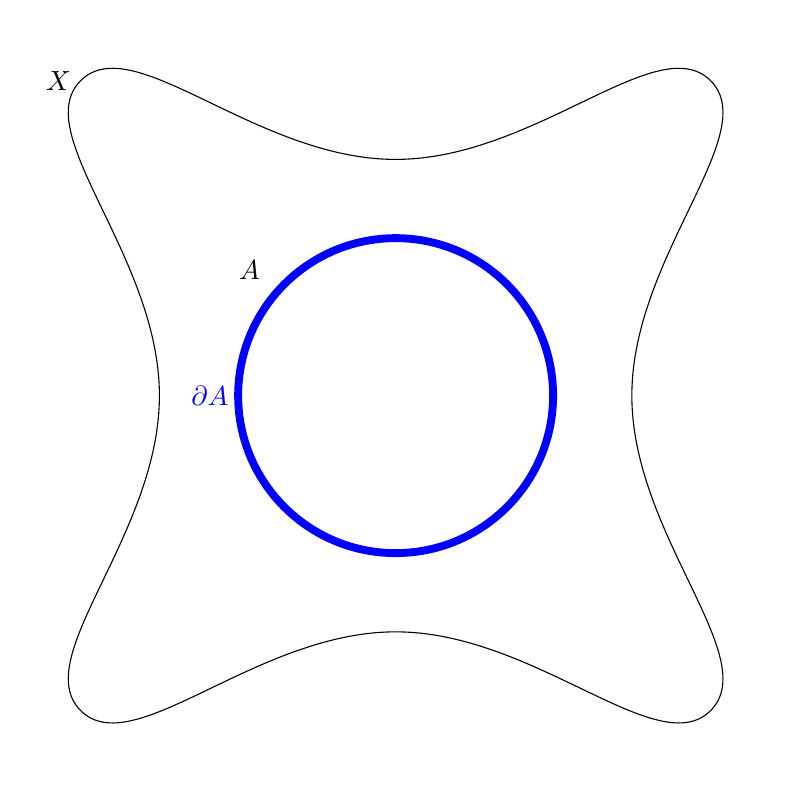
\begin{tikzpicture}[scale=2]
        \draw plot[smooth cycle, tension=0.8] coordinates {(2,2) (1.5,0) (2,-2) (0,-1.5) (-2,-2) (-1.5,0) (-2,2) (0,1.5)};
        \node[left] at (-2,2){$X$};
        \draw[radius=1, line width=0.1cm, blue](0,0) circle;
        \node[left] at (-0.8,0.8){$A$};
        \node[left, blue] at (-1,0){$\partial A$};
    \end{tikzpicture}
\end{center}

\vspace*{13mm}

We also need to stay away from $\partial A$. Suppose $\exists y\in B(x,\varepsilon)$ such that $y\in\partial A$

Then $y\in\partial A$ and by definition, $\forall\delta>0$, 
\begin{align*}
    B(y,\delta)\cap A\neq\emptyset\text{ and }B(y,\delta)\cap A^{c}\neq\emptyset
\end{align*}
But $d(x,y)=\varepsilon^{*}<\varepsilon$. Consider then the ball $B(y,\frac{\hat{\varepsilon}}{2})$ where $\hat{\varepsilon}=\min\{\varepsilon^{*},\varepsilon-\varepsilon^{*}\}$. Then the $B(y,\hat{\varepsilon})\subseteq B(x,\varepsilon)$ but $B(y, \hat{\varepsilon})\cap A\neq\emptyset$ which is a \textbf{\underline{contradiction}} as $B(x,\varepsilon)\subseteq A^{c}$. We cannot simultaneously intersect with $A$ and lie entirely within $A^{c}$.
\end{multicols}

Recall:
\begin{itemize}[label=\empty]
    \item ($X$, $d$) \& $A\subseteq X$ we associate with $A$, a set $\overline{A}$ known as the closure of $A$, where
    \subitem $\overline{A}:=A\cup\partial A$ ($\partial A$ is the set of all boundary points of $A$)
    \subitem $\overline{A}$ is closed. ($F\subseteq X$ is closed $\iff\partial F\subseteq F$.)
\end{itemize}

\begin{itemize}
    \item[Example:] In the metric space $(\mathbb{R}^{n}, d_{2})$, where $\mathbb{R}^{n}$ is Euclidean $n$-space and $d_{2}(x,y)=\sqrt{\sum^{n}_{i=1}|x_{i}-y_{i}|^{2}}$,
    \subitem $\overline{B(x,r)}=\overline{B}(x,r)$. In other words, the closure of the open ball centred at $x$ of radius $r$ is the closed ball.
    \item[Note:] This is not true in general. $\exists (x,d)$ such that $\overline{B(x,r)}\neq\overline{B}(x,r)$
\end{itemize}

\begin{multicols}{2}
    \begin{tikzpicture}[scale=2]
        \draw[-](-1,0)--(1,0);
        \draw[-](0,-1)--(0,1);
        \draw[dashed, radius=1.2](0,0) circle;
        \draw[->](0,0)--(1.15,0.2);
        \draw[-](-1.4,-1.4)--(1.4,1.4);
        \node[left] at (1,0.3){$r$};
        \draw[dashed, radius=0.3](0.8485281374,0.8485281374) circle;
        \node[right] at (1.4,1.4){$y$};
        \node[below] at (0.1,0.01){$x$};
    \end{tikzpicture}

    \begin{itemize}
        \item[Observation:] No point in $B(x,r)=\{y\in\mathbb{R}^{n}:d_{2}(x,y)<r\}$ is a boundary point; indeed they are all interior points.
        \item[Recall:] $\partial A$, $A^{o}$ \& $A^{e}$ are all pairwise disjoint.
        
    \end{itemize}
    Sufficient to show
        \begin{align*}
            \boxed{\partial B(x,r)=\{y\in\mathbb{R}^{n}:d_{2}(x,y)=r\}\subseteq \overline{B}(x,r):=C}
        \end{align*}
    Straight forward to show that any $y\in\mathbb{R}^{n}$ for which $d_{2}(x,y)>r$ in in the exterior of $B(x,r)$.
\end{multicols}
We know that $\underline{r}\in Ly$ can be written in the form $\underline{r}=x+\lambda(y-x)$ where $\lambda\in\mathbb{R}$. If $\lambda\in(-1,1)$ then $\underline{r}\in B(x,r)$ \& $\lambda\notin(-1,1)$ then $\underline{r}\notin B(x,r)$ \& further $\underline{r}(1)=\underline{x}+1(\underline{y}-\underline{x})=\underline{y}$.

Let $\varepsilon>0$ be given. Choose $\delta:=\min\{\frac{\varepsilon}{2},\frac{r}{2}\}$. Then $\underline{r}(\delta)=\underline{x}+\delta(\underline{y}-\underline{x})\in B(x,r)$ \& $\underline{r}(1+\delta)=\underline{x}+(1+\delta)(\underline{y}-\underline{x})\in B(x,r)^{c}$. From this we can deduce (by alternating $\delta$ slightly) that $B(y.\delta)\cap B(x,r)\neq\emptyset$ and $B(y,\delta)\cap B(x,r)^{c}\neq\emptyset$ which together define a boundary point.
\begin{itemize}
    \item[Note:] $\boxed{\overline{B}(x,r)=B(x,r)\cup C.}$ 
\end{itemize}


TBC...


%------------------------------------Bibliography--------------------------------------------%
\newpage
\section{References}
\begin{thebibliography}{1}
\bibitem{Book 1}
O'Searcoid, M. (2006). Metric Spaces. 1st ed. London: Springer Nature.

\bibitem{Book 2}
Shirali, S. (2005). Metric Spaces. 1st ed. London: Springer Nature.

\bibitem{Book 3}
Hart, F.M. (2001) Guide to analysis / F. Mary Hart. 2nd ed. Basingstoke:, Palgrave.

\bibitem{Book 4}
Alcock, L. (2014) How to think about analysis /. Oxford University Press,.

\bibitem{Book 5}
Hirst, K.E. (1995) Numbers, sequences and series / Keith E. Hirst. London:, E Arnold.

\end{thebibliography}

\end{document}
